\documentclass[11pt]{article}
\usepackage[margin=1in]{geometry}
\usepackage{amsmath,amssymb,amsthm,booktabs,tikz}
\usepackage[hyperfootnotes=false]{hyperref}
\hypersetup{colorlinks=true,linkcolor=blue,citecolor=blue,urlcolor=blue,pdfauthor={GPT-6 Astra},pdftitle={One pitch shifts in six note homometry}}
\newtheorem{theorem}{Theorem}
\newtheorem{lemma}[theorem]{Lemma}
\newtheorem{corollary}[theorem]{Corollary}
\newtheorem{remark}[theorem]{Remark}
\newcommand{\Z}{\mathbb Z}
\newcommand{\ind}{\mathbf 1}
\DeclareMathOperator{\ord}{ord}
\title{One pitch shifts in six note homometry}
\author{GPT-6 Astra}
\date{13 October 2026}
\begin{document}
\maketitle
\begingroup\renewcommand{\thefootnote}{}\footnotetext{Project AI-author label; no runtime-model identity or OpenAI affiliation is asserted.}\endgroup
\begin{abstract}
We study pairs of six-element subsets of a finite cyclic group that have the same difference multiset, are inequivalent under translation and reflection, and share five elements after suitable alignment. Such a pair exists in $\Z/n\Z$ exactly when $n\ge12$ and either $3\mid n$ or $4\mid n$. A periodic-indicator criterion yields four exhaustive structural templates. We also classify the subfamily whose exchanged interval has additive order four: its number of unordered pairs of bracelet classes is $2\lfloor s/2\rfloor$ when $n=8s$, and zero otherwise. These statements concern a restricted stratum of six-note homometry; they do not classify all hexachords or whole homometry classes.
\end{abstract}
\paragraph{Verification status.} The six-note existence theorem and the general exchange obstructions have passed Lean 4.32.2 with an exact statement and axiom audit. An independent fresh-object replay of all 33 modules and a separately expanded elementary statement also passed. The order-four enumeration has an independent mathematical audit and bounded exact checks, but is not yet formalized in Lean. The literature review is unfinished, so no priority or publication-level novelty claim is made.

\section{Definitions and the scope of the result}
For a finite subset $A$ of an abelian group, write
\[
 \nu_A(t)=\#\{(u,v)\in A^2:u-v=t\}.
\]
Two sets are \emph{homometric} when their functions $\nu$ agree. For equal-cardinality subsets of $\Z/n\Z$, this is equivalent to equality of the multiset of unordered Lee distances. A \emph{bracelet} is an equivalence class under translations $x\mapsto x+t$ and reflections $x\mapsto t-x$.

A pair is \emph{strict} if its two bracelets differ. A \emph{one-pitch shift} means replacing just one element: after translation its representatives have the form
\begin{equation}\label{eq:normal}
 A=C\cup\{0\},\qquad B=C\cup\{d\},\qquad d\ne0,\quad 0,d\notin C.
\end{equation}
For six notes, $|C|=5$. The terminology and examples of this operation predate the present investigation, notably Althuis--G\"obel~\cite{AG}. Erickson--Jones~\cite{EJ} leave the general classification for six or more points open. Our restriction to representatives of the form~\eqref{eq:normal} is essential.

\section{The periodic indicator criterion}
\begin{lemma}\label{lem:criterion}
Let $G$ be a finite abelian group and let $A,B,C,d$ satisfy~\eqref{eq:normal}. Put $c=\ind_C$ and $f(x)=c(x)-c(d-x)$. Then $A,B$ are homometric if and only if
\[
 f(x+d)=f(x)\quad\text{for every }x\in G.
\]
\end{lemma}
\begin{proof}
The ordered pairs internal to $C$, and the self-pair contributed by the inserted element, cancel. For every $t$,
\begin{align*}
\nu_A(t)-\nu_B(t)
 &=c(t)+c(-t)-c(d+t)-c(d-t)\\
 &=f(t)-f(t+d).
\end{align*}
This proves both implications without division, including when $t$ is a torsion element.
\end{proof}

\begin{lemma}\label{lem:decomp}
Write $R(x)=d-x$, $H=\langle d\rangle$, and
\[
 P=C\setminus R(C),\qquad Q=C\cap R(C).
\]
Then $A,B$ are homometric if and only if $P$ is a union of $H$-cosets. The decomposition $C=P\sqcup Q$ is canonical, and satisfies
\[
 P\cap R(P)=\varnothing,\qquad R(Q)=Q,\qquad
 Q\cap(P\cup R(P))=\varnothing.
\]
Conversely any such $P,Q$ avoiding $0,d$ produce a homometric pair.
\end{lemma}
\begin{proof}
The function $f$ is $1$ on $P$, $-1$ on $R(P)$, and zero elsewhere. A $d$-periodic $f$ has $H$-invariant level sets. Conversely, $R$ carries $H$-cosets to $H$-cosets, so invariance of $P$ implies invariance of all three level sets. The remaining statements follow from $R^2=\mathrm{id}$.
\end{proof}

\begin{corollary}\label{cor:torsion}
If a strict homometric pair of $k$-element sets differs in one point, its exchanged element $d$ has order $m$ satisfying
\[
 2\le m\le k-2.
\]
The ambient finite abelian group also satisfies $|G|\ge k+m+1$. If $k$ and $m$ are both even and the group is $\Z/n\Z$, then $2m\mid n$.
\end{corollary}
\begin{proof}
If $P=\varnothing$, the reflection $R$ maps $A$ to $B$, contradicting strictness. Thus $P$ contains an $H$-coset, so $m\le|C|=k-1$. Equality forces $C$ to be exactly one $H$-coset, in which case translation by $d$ maps $A$ to $B$. Therefore $m\le k-2$.

By definition of $P$, its reflection $R(P)$ is disjoint from $C$. Both $C$ and $R(P)$ avoid $0,d$, because $R$ exchanges these endpoints. Thus $C$, $R(P)$, $\{0\}$, and $\{d\}$ are pairwise disjoint. Since $|R(P)|=|P|\ge m$, we obtain $|G|\ge |C|+m+2=k+m+1$.

If $k,m$ are even, then $|P|$ is even and $|Q|=k-1-|P|$ is odd. The involution $R$ on $Q$ has a fixed point, so $2r=d$ for some $r$. Write $n=mg$ and $d=gu$ with $\gcd(u,m)=1$. Since $m$ is even, $u$ is odd. Solvability of $2r=d$ modulo the even integer $n$ forces $d$ even, hence $g$ even. Thus $2m\mid n$.
\end{proof}

\section{The six note existence theorem}
\begin{theorem}\label{thm:existence}
Strict one-pitch-shift homometric pairs of six-note bracelets in $\Z/n\Z$ exist if and only if
\[
 n\ge12\quad\text{and}\quad (3\mid n\text{ or }4\mid n).
\]
\end{theorem}
\begin{proof}
Corollary~\ref{cor:torsion} leaves $m=2,3,4$ and gives $n\ge m+7$. If $m=2$, then $n\ge9$ and $4\mid n$, hence $n\ge12$. If $m=3$, then $n\ge10$ and $3\mid n$, again giving $n\ge12$. If $m=4$, then $n\ge11$ and $8\mid n$, so $n\ge16$. This proves the necessity, including the lower bound, without finite enumeration.

For $n=4q$, $q\ge3$, take $d=2q$ and
\[
 C=\{1,2q+1,q-1,q,q+1\}.
\]
The set $\{1,2q+1\}$ is an $H$-coset, and the other three points are invariant under $R$. Lemma~\ref{lem:decomp} gives homometry. In ascending circular order, the gap sequences of $A,B$ are
\[
\begin{array}{ll}
 A:&(1,q-2,1,1,q,2q-1),\\
 B:&(q-2,1,1,q-1,1,2q).
\end{array}
\]
Their maximum gaps differ, proving strictness.

For $n=3q$, $q\ge5$, take $d=q$ and
\[
 C=\{1,q+1,2q+1,2,q-2\}.
\]
The first three points form an $H$-coset, while the last two are exchanged by $R$. The gap sequences are
\[
\begin{array}{ll}
 A:&(1,1,q-4,3,q,q-1),\\
 B:&(1,q-4,2,1,q,q).
\end{array}
\]
The largest gap $q$ occurs once in $A$ and twice in $B$, proving strictness. The remaining modulus $12$ is already covered by the first construction.
\end{proof}

\begin{corollary}\label{cor:templates}
Every strict six-note one-pitch-shift pair admits the canonical decomposition of Lemma~\ref{lem:decomp} in one of the following four sizes:
\begin{center}
\begin{tabular}{ccc}\toprule
Order of $d$ & Number of $H$-cosets in $P$ & $|Q|$\\\midrule
2&1&3\\2&2&1\\3&1&2\\4&1&1\\\bottomrule
\end{tabular}
\end{center}
Conversely the conditions of Lemma~\ref{lem:decomp} suffice for homometry in each row, but a dihedral noncongruence test is still required in general.
\end{corollary}
\begin{proof}
The order is at most four, $P$ is nonempty with cardinality divisible by that order, and $|P|+|Q|=5$.
\end{proof}
\begin{remark}
The noncongruence condition cannot simply be omitted. In $\Z/12\Z$, take $d=6$ and $C=\{1,3,4,7,10\}$. This has $P=\{1,4,7,10\}$ and $Q=\{3\}$, yet $B=A+3$. The templates are exhaustive structural candidates, not four automatically strict families.
\end{remark}

\section{Exact enumeration for exchange order four}
\paragraph{Construction attribution.} The regular polygon plus two-point construction underlying this stratum is classical: Goyette~\cite[pp.~75--76]{Goyette} attributes it to Patterson~\cite[p.~199]{Patterson}. We claim no novelty for that construction. The proposed contribution in this section is its exhaustive one-exchange characterization and irredundant dihedral quotient count. The original Patterson page still requires direct inspection.
\begin{theorem}\label{thm:four}
Let $h_4(n)$ count unordered pairs of distinct six-note bracelet classes that admit a one-pitch-shift realization with exchanged interval of additive order four. Then
\[
 h_4(n)=\begin{cases}
 2\lfloor s/2\rfloor,&n=8s,\\
 0,&8\nmid n.
 \end{cases}
\]
For $n=8s$, irredundant representatives are indexed by
\[
 r\in\{s,5s\},\qquad 1\le a\le\lfloor s/2\rfloor,
\]
and are
\[
 H=\{0,2s,4s,6s\},\quad P=a+H,\qquad
 A=P\cup\{0,r\},\quad B=P\cup\{2s,r\}.
\]
\end{theorem}
\begin{proof}
Corollary~\ref{cor:torsion} requires $n=8s$. Reflection normalizes the exchanged interval to $d=2s$. Corollary~\ref{cor:templates} gives one $H$-coset $P=a+H$ and a singleton $Q=\{r\}$ with $2r=d$. Thus $r=s$ or $5s$. The condition $P\cap R(P)=\varnothing$ excludes exactly $a=0,s$ modulo $2s$; these exclusions also give all required disjointness.

Each six-set contains a unique full $H$-coset. Indeed distinct cosets are disjoint and only two points remain outside $P$. Consequently every dihedral equivalence carries the four-point coset to its counterpart and the residual two-point set to its counterpart.

For a map from $A$ to $B$ the only possible maps of residual pairs are translation by $r$ and reflection $x\mapsto d-x$. Translation by $r$ does not preserve $P$, because $r\notin H$. The reflection preserves $P$ only when $2a=0$ modulo $2s$, precisely the excluded parameters. All these pairs are therefore strict.

The residual pair has Lee distance $s$ in the family $r=s$, and $3s$ in the family $r=5s$. This separates the two families under all equivalences, including independent equivalences of each bracelet.

Fix $r$. An equivalence between $A_a$ and $A_b$ must either fix the residual pair $\{0,r\}$ pointwise or interchange it. These give respectively $b=a$ and $b=s-a$ modulo $2s$. Reflection $x\mapsto d-x$ sends $B_a$ to $A_{-a}$. Thus equality of unordered bracelet pairs gives exactly the parameter orbit generated by
\[
 a\longmapsto-a,\qquad a\longmapsto a+s.
\]
Modulo $s$, with zero excluded, inversion has representatives $1\le a\le\lfloor s/2\rfloor$. There are $\lfloor s/2\rfloor$ pairs for each of the two values of $r$.
\end{proof}
\begin{remark}
This count quotients each chord independently by translation and reflection. It does not count simultaneous orbits of marked configurations. A counted pair may belong to a larger homometry class, or admit a second one-pitch-shift realization of another exchange order.
\end{remark}

\section{Examples and verification}
For $n=16$ the order-four theorem supplies exactly two pairs, represented by
\[
\begin{array}{ll}
\{0,1,2,5,9,13\},&\{1,2,4,5,9,13\},\\
\{0,1,5,9,10,13\},&\{1,4,5,9,10,13\}.
\end{array}
\]
For a familiar twelve-tone example, the first existence construction gives
\[
 A=\{0,1,2,3,4,7\},\qquad B=\{1,2,3,4,6,7\}.
\]
Only the note $0$ moves, to $6$; five pitch classes remain fixed.

\begin{center}
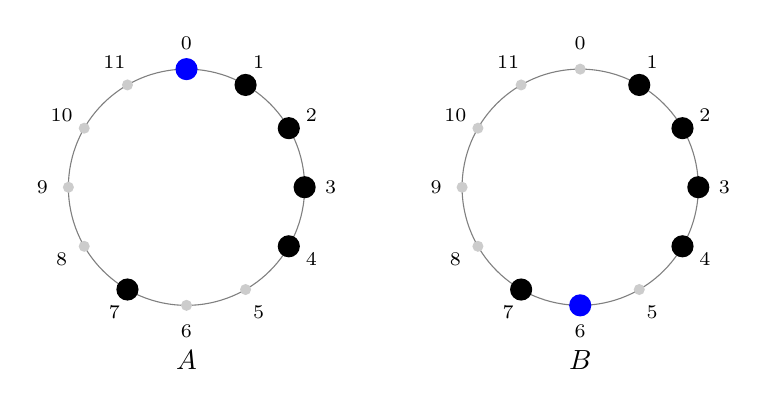
\begin{tikzpicture}[scale=1]
\foreach \offset/\lab/\pts in {0/$A$/\empty,5/$B$/\empty} {
\begin{scope}[xshift=\offset cm]
\draw[gray] (0,0) circle (1.5);
\foreach \i in {0,...,11} {\fill[gray!40] ({90-30*\i}:1.5) circle (2pt);\node[font=\scriptsize] at ({90-30*\i}:1.83) {\i};}
\foreach \i in {1,2,3,4,7} \fill[black] ({90-30*\i}:1.5) circle (4pt);
\node at (0,-2.2) {\lab};
\end{scope}}
\fill[blue] (90:1.5) circle (4pt);
\begin{scope}[xshift=5cm]\fill[blue] (-90:1.5) circle (4pt);\end{scope}
\end{tikzpicture}
\end{center}

A direct Lee-distance enumeration independently checked all normalized one-pitch shifts for $6\le n\le24$. A separate canonicalization of the order-four parameter family checked the formula through $n=160$. These are consistency checks; neither the mathematical existence proof nor its Lean proof depends on them.

The checked Lean theorem is \texttt{OnePitchShift.six\_note\_one\_exchange\_existence\_iff}. Its left side quantifies over actual finite subsets $A,B\subseteq\Z/n\Z$ with $|A|=|B|=6$ and $|A\cap B|=5$, equality of directed difference multiplicities, and no translation/reflection equivalence. The right side is exactly $n\ge12$ and $(3\mid n\text{ or }4\mid n)$. Translation invariance and the passage to the normalized common-set form are proved in the source. The two parametric witnesses are verified for all parameters; their formal noncongruence proofs exclude the twelve possible affine maps rather than introducing circular-gap infrastructure.

The pinned library is Mathlib commit \texttt{905b95818eb32af7874a58b427f50c1711a5e96c}. The audited dependencies use only \texttt{propext}, \texttt{Classical.choice}, and \texttt{Quot.sound}; there are no custom axioms, proof placeholders, or native decision certificates. The independent replay rebuilt all 33 local modules into a fresh object directory, omitted the original project objects, and checked a separately written statement with expanded finite-set definitions. Its report and hash receipts accompany the sources. Cached standard-library and Mathlib objects form the pinned trusted baseline. The order-four quotient theorem is a separate, not-yet-formalized result.

\section{Prior work and remaining questions}
One-pitch shifts and sufficient constructions are established ideas. Althuis--G\"obel~\cite{AG} study the operation for four- and five-note families. Collins~\cite{Collins} proves a one-step obstruction, an earlier special case of the generating-displacement restriction. Masai--McShane~\cite{MM} give constructions using invariant components and involutive isometries. Goyette's dissertation~\cite{Goyette}, Chapter~3, develops cyclic-component transformations. Its pp.~75--76 explicitly attribute the regular polygon plus two-point construction to Patterson~\cite[p.~199]{Patterson}; this construction is therefore prior art, not a candidate contribution of this note. These sources must be distinguished from an exhaustive necessity statement or an irredundant count.

For the exact existence iff, the relevant distinction is between supplying examples and excluding every other modulus. The inspected Althuis--G\"obel families concern four and five notes; Collins addresses a one-step obstruction; the cited invariant-component methods provide constructions. None of those inspected statements is the exact all-modulus six-note criterion of Theorem~\ref{thm:existence}. This comparison is limited to material actually inspected. Erickson--Jones leaving the unrestricted six-note problem open does not by itself establish novelty of this restricted theorem.

The candidate contributions here are the six-note arithmetic existence criterion and the exact order-four quotient. Direct inspection of Patterson's p.~199, Soderberg's original dual-inversion paper, and Collins's full report is still needed before asserting novelty. Relevant construction sections of Goyette's full dissertation have now been inspected. The general six-note classification in~\cite{EJ}, the irredundant enumeration of the other one-pitch-shift templates, and a Lean verification of the order-four enumeration remain open tasks in this project. The exact six-note one-exchange existence theorem is now formalized, but whether that exact arithmetic criterion was previously published remains unresolved.

\begin{thebibliography}{9}
\bibitem{EJ} W. Q. Erickson and N. B. Jones, \emph{Homometric subsets of $\Z_n$ with cardinality 5: classification and enumeration}, arXiv:2412.08997v4 (27 August 2026), \href{https://arxiv.org/html/2412.08997v4#S5}{Section 5}.
\bibitem{AG} T. A. Althuis and F. G\"obel, \emph{Z-related pairs in microtonal systems}, University of Twente Memorandum 1524 (2000), \href{https://ris.utwente.nl/ws/portalfiles/portal/5115044/1524.pdf}{primary report}.
\bibitem{Collins} N. Collins, \emph{Transposition Invariance and Parsimonious Relation of Z Sets}, unpublished report (2001, revised 2002), \href{https://composerprogrammer.com/research/selftransposingz.pdf}{author-hosted report}. Indexed primary text inspected; complete file not retrieved.
\bibitem{MM} H. Masai and G. McShane, \emph{Isospectral configurations in Euclidean and hyperbolic geometry}, arXiv:2308.12109, \href{https://macbuse.github.io/MC0726.pdf}{author manuscript}, Section 8.
\bibitem{Goyette} J. Goyette, \emph{The Z-Relation in Theory and Practice}, Ph.D. dissertation (2012), \href{https://urresearch.rochester.edu/fileDownloadForInstitutionalItem.action?itemFileId=76476&itemId=24908}{full dissertation}. Relevant sections of the full \href{https://urresearch.rochester.edu/fileDownloadForInstitutionalItem.action?itemFileId=76476\&itemId=24908}{dissertation} have been inspected.
\bibitem{Patterson} A. L. Patterson, \emph{Ambiguities in the X-Ray Analysis of Crystal Structures}, Physical Review 65 (1944), 195--201, \href{https://doi.org/10.1103/PhysRev.65.195}{doi:10.1103/PhysRev.65.195}. Construction attribution verified through Goyette; original p.~199 not yet inspected.
\bibitem{JJ} F. Jedrzejewski and T. Johnson, \emph{The Structure of Z-Related Sets}, Mathematics and Computation in Music (2013), 128--137, \href{https://arxiv.org/abs/1304.6608}{arXiv:1304.6608}.
\end{thebibliography}
\end{document}
